\chapter{Case study}

In this chapter, a study case is presented to understand the concepts proposed
method.

\section{Motivation and objectives}

Our motivation begins to know if a user model in combination with
other techniques such as usability or fuzzy logic increases the participation of users in a
given Web-based IEC application. It is well know that one of the main
problems in these systems is fatigue, who is the cause by the large
amount of individual evaluations
that the user need to preform and consequently their participation decreases.

Our approach goes with the sense of increasing the participation of the users
within these applications, providing to them very simple tasks to execute in order to
capture their attention as well as to know their behavior.


Since we have described that the main approach is to increase the participation
of users, in order to measure these results and to be able to demonstrate
if the participation
of these users increase, it was necessary to build a study
case where an evolutionary art application is involved within an interactive
evolutionary system which we call EvoDrawings. This application was modified in
order to obtain three versions of this one, which were labeled with the names
ED01, ED02, ED03. The objective is to extract data from each of the different
versions and then quantify and compare which of these had the best result in the
participation of the users.

\section{EvoDrawings} EvoDrawings is based on the EvoSpace-i framework and
consequently uses the same architecture which is presented in Figure
\ref{fig:ESFramework}. This architecture have the individual block which
contains different information, including the chromosome that represents the
digital painting. Technically the individual is an associative arrangement
(dictionary) where an abstract collection of keys and values is stored with a
one-to-one association. Where keys represent a specific property in each object
and the values are different types of data, such as lists, tuples, numbers,
strings and dictionaries.

\begin{figure*}
\captionsetup{justification=centering,margin=2cm}
\centering
\setlength\fboxsep{0pt}
\setlength\fboxrule{0.7pt}
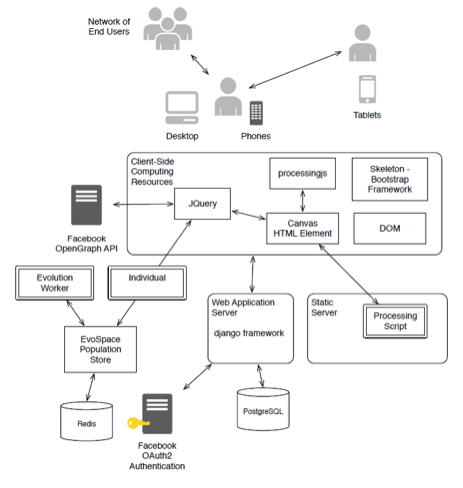
\includegraphics[width=8cm,height=8cm,keepaspectratio]{img/ESFramework.png}
\caption{EvoSpace-i framework.}
\label{fig:ESFramework}
\end{figure*}


The individual has the following fields, shown in Figure \ref{fig:individual_dic}.
The field is represented by a single string for each object. The chromosome
field represented by a string, which for EvoDrawing represents an array of 15
numerical characters which define the behavior of the digital drawing. The
fitness field is defined by a dictionary, this field contains the information of
users evaluations as well as the creation date as a timestamp. The field called
views is determined by a string and represent the number of times they have seen
the individual. The keys called mom and dad define where the individual comes
from. The GeneticOperator field is a string that specifies the genetic operator
produced.

\begin{figure*}
\captionsetup{justification=centering,margin=2cm}
\centering
\setlength\fboxsep{0pt}
\setlength\fboxrule{0.7pt}
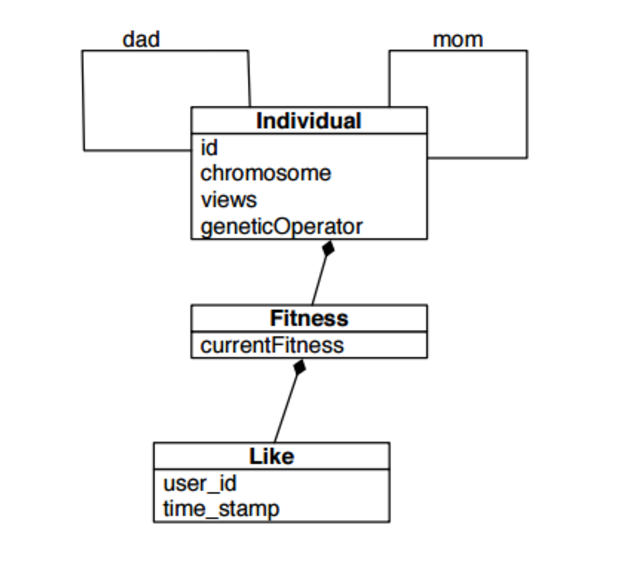
\includegraphics[width=8cm,height=8cm,keepaspectratio]{img/individual_dic.png}
\caption{Chromosome representation.}
\label{fig:individual_dic}
\end{figure*}

\subsection{Processing Script}
It is necessary to explain how the animation
that the users visualize works. EvoSpace-i uses processing script in order to do
the rendering of the individuals which contain the behavior of the figures. This
application can run in browsers that are compatible with HTML 5, this is due to
the use of a JavaScript library called processingscriptjs that is in charge of
communicating with the base script and thus perform the render on HTML 5 canvas
in The EvoDrawings application.

\subsection{Fitness}
The fitness assignment for each individual is given by the
evaluations of users. EvoDrawings has reviews when users give their
rating. We can see this rating on Figure \ref{fig:individual_dic} of the
interface that EvoDrawings uses in all its variations. This rate ranges from 1
star to 5 stars, which defines the user's liking for the digital drawing
presented by EvoDrawings. When users evaluate a sample of individuals, some of
these will not receive any evaluation. The view property, it increases by 1 when
it is viewed. Internally, a fitness calculation is used defined by the following
equation:

\begin{equation}\label{eq:fitfunc01}
\displaystyle fitness=\frac{\sum_{i=0}^{n}x_{i}+ 1}{\sum_{i=0}^{n}v_{i} + 1}
\end{equation}

$i$ represents the individual's.
$x$ is the range that individuals received when evaluated by users.
$v$ are the views that users have viewed individuals.

The above is used in version ED01. For the next two versions we use a different
defined fitness based on the behavior that users perform within EvoDrawings,
such as assigned tasks, the logging action in order to start evaluating
individuals, individuals evaluation, creating collections for later store
individuals and finally view the public individuals of friends who are
participating in the application.

For ED02 we use a fuzzy inference system consisting of two inputs and one
output. Entries are defined by preference and experience. The preference is the
range of stars from 1 to 5 and are the evaluations that users give to the
presented digital drawing, and are represented with triangular membership
functions called high, medium and low. In the same way the input experience is
defined by the tasks performed and it has the range of 1 to 100, each task
receives points until reaching a threshold of 100 points where the user is
considered as an expert within the application. This input is also represented
by triangular membership functions called high, medium, low. Finally we have the
output called fuzzy\_rate in a range of 1 to 100, defined by triangular
membership functions called bad, normal, good. This fuzzy system consists of 9
if-then rules:

\begin{enumerate}
	\item \textit{If \textbf{preference} is low and
		\textbf{experience} is low then \textbf{fuzzy\_rate} is bad.}
	\item \textit{If \textbf{preference} is mid and
		\textbf{experience} is low  then \textbf{fuzzy\_rate} is bad.}
	\item \textit{If \textbf{preference} is high and
		\textbf{experience} is low  then \textbf{fuzzy\_rate} is normal.}
	\item \textit{If \textbf{preference} is low and
		\textbf{experience} is mid then \textbf{fuzzy\_rate} is bad.}
	\item \textit{If \textbf{preference} is mid and
		\textbf{experience} is mid  then \textbf{fuzzy\_rate} is normal.}
	\item \textit{If \textbf{preference} is high and
		\textbf{experience} is mid  then \textbf{fuzzy\_rate} is good.}
	\item \textit{If \textbf{preference} is low and
		\textbf{experience} is high then \textbf{fuzzy\_rate} is normal.}
	\item \textit{If \textbf{preference} is mid and
		\textbf{experience} is high  then \textbf{fuzzy\_rate} is good.}
	\item \textit{If \textbf{preference} is high and
		\textbf{experience} is high  then \textbf{fuzzy\_rate} is good.}

\end{enumerate}

The fitness function is given by the following equation:

\begin{equation}\label{eq:fitfunc02}
\displaystyle fitness=\frac{\sum_{i=0}^{n}x_{i}+f(y_{i})}{\sum_{i=0}^{n}f(y_{i})}
\end{equation}

$i$ represents the individual's. x is the range that users give to individuals..
$f(y_i)$ represents a fuzzy function composed of a fuzzy inference system and is
represented by the equation \ref{eq:fuzzyFunc}.

\begin{equation}\label{eq:fuzzyFunc}
\displaystyle y=fr(x,e)
\end{equation}


$fr$ represents the fuzzy rate. $x$ it remains the range that users give
according to their preferences to individuals. $e$  is the experience that is
defined by the activity that the user is doing within the application. The fuzzy
inference system of it is a Mamdani type composed of two inputs that are  $x,e$
and a fuzzy rate output as shown in Figure \ref{fig:fis_01}.

\begin{figure*}
\captionsetup{justification=centering,margin=2cm}
\centering
\setlength\fboxsep{0pt}
\setlength\fboxrule{0.7pt}
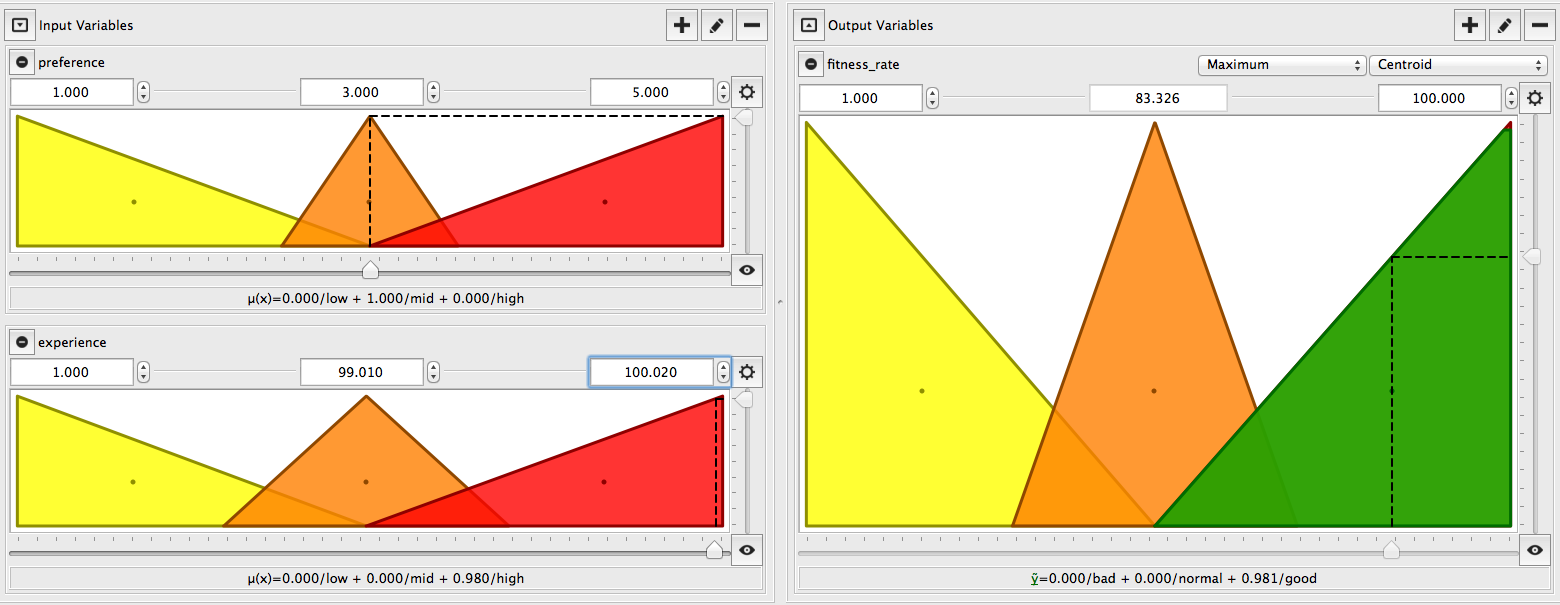
\includegraphics[width=12cm,height=10cm,keepaspectratio]{img/fuzzy_system_2_1.png}
\caption{Chromosome representation.}
\label{fig:fis_01}
\end{figure*}

For ED03 the fitness function is given by the same equation as ED02 the
difference relies in the inputs of the fuzzy function, for this case a new input
is added with the name of ranking. This new input is the given by the
cardinality of the graph of the user model for each user. here is the fuzzy
function for ED03.

\begin{equation}\label{eq:fuzzyFunc2}
\displaystyle y=fr(x,e,r)
\end{equation}

$fr$ represents the fuzzy rate.
$x$ it remains the range that users give according to their preferences to individuals.
$e$  is the experience that is defined by the
activity that the user is doing within the application.
$r$ is the ranking the user within the graph model.
 The fuzzy inference system it is a Mamdani type composed of three inputs that
are  $x,e, r$ and a fuzzy rate output as shown in Figure \ref{fig:fis_02}.

\begin{figure*}
\captionsetup{justification=centering,margin=2cm}
\centering
\setlength\fboxsep{0pt}
\setlength\fboxrule{0.7pt}
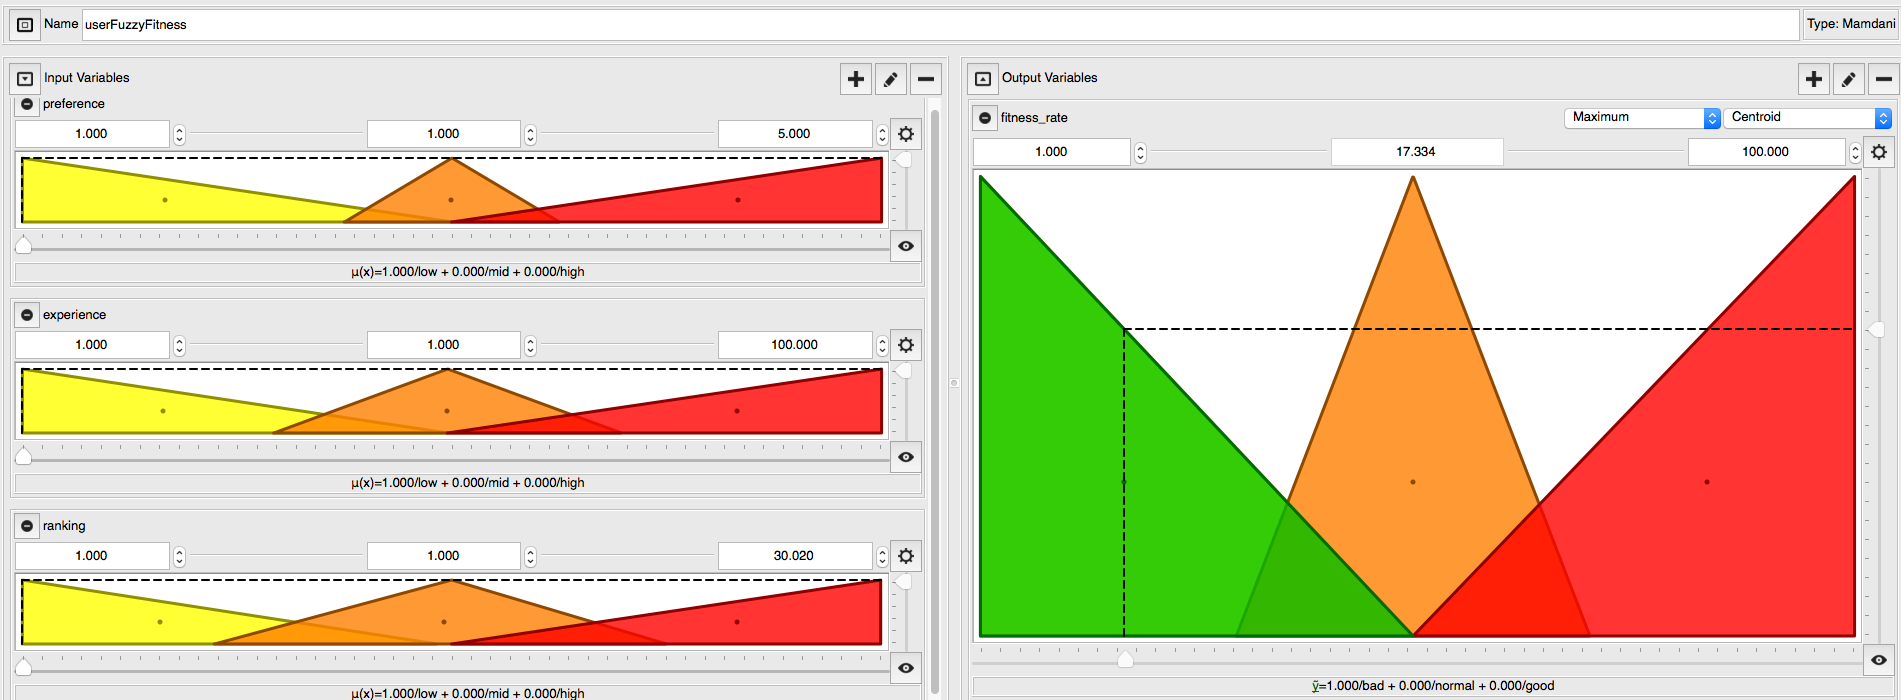
\includegraphics[width=12cm,height=10cm,keepaspectratio]{img/fuzzySys.png}
\caption{Fuzzy inference system for ED03.}
\label{fig:fis_02}
\end{figure*}


\subsection{Configurations.}

Previously we mentioned that EvoDrawings is an application of evolutionary art
within an evolutionary system with the aim of being able to prove the increase
of the participation of the users. To prove this hypothesis within this thesis,
3 different versions of EvoDrawing were designed. The EvoDrawing versions and
the results of the experiments were compared to each other. All experiments and
comparisons were performed on equal data, parameters and users.

For ED03 the initial configuration of our evolutionary algorithm in this version
is the following:

\begin{enumerate}
	\item  \textbf{We have an initial population of 80 individuals.}

	\item  \textbf{An evolution parameter is 8 evaluations.}

	\item  \textbf{A mutation parameter of }
	\item  \textbf{With random selection between competition.}
	\item  \textbf{One horizontal genetic crossing Operator.}
	\item  \textbf{The fitness is given by the equation \ref{eq:fitfunc01}.}
\end{enumerate}

For the interface in this version there is an easy-to-use Web interface for
users to evaluate  individuals. Figure\ref{fig:UI_01} shows the navigation
bar that has the functionality for logging in to the application.
Once logged in with a Facebook account, an avatar appears in the navigation bar
as well as the functionality to exit the application through a logout button. Also
within this interface exists the visual element \'Friends\' where all the friends
that are participating in the application appear, this element also has the
functionality to be able to see the public collections that the these friends have.
Continuing with the explanation of the interface we have the \'Collections\' panel
which shows a list of collections that users have created and saved, as well as
the functionality to create new collections. Within this we have
an \'About this\' section where users can read general information about the
system. Users can evaluate individuals throu a
visual canvas element that shows the behavior of the individual subject to
evaluation (animation) and at the bottom is given the ability to evaluate the
individual with a range of stars where one star means the user did not like it
very much and five stars mean the user like it too much. Now at the bottom of
the star range we have a button that provides the functionality of being able to
add this individual to a collection. At
the top of the star rank is a label with the legend that says 'Click here to
see my DNA History' this takes the user to a detail page about the individual that is
been evaluated, this is shown
in Figure\ref{fig:dna}.

\begin{figure*}
\captionsetup{justification=centering,margin=2cm}
\centering
\setlength\fboxsep{0pt}
\setlength\fboxrule{0.7pt}
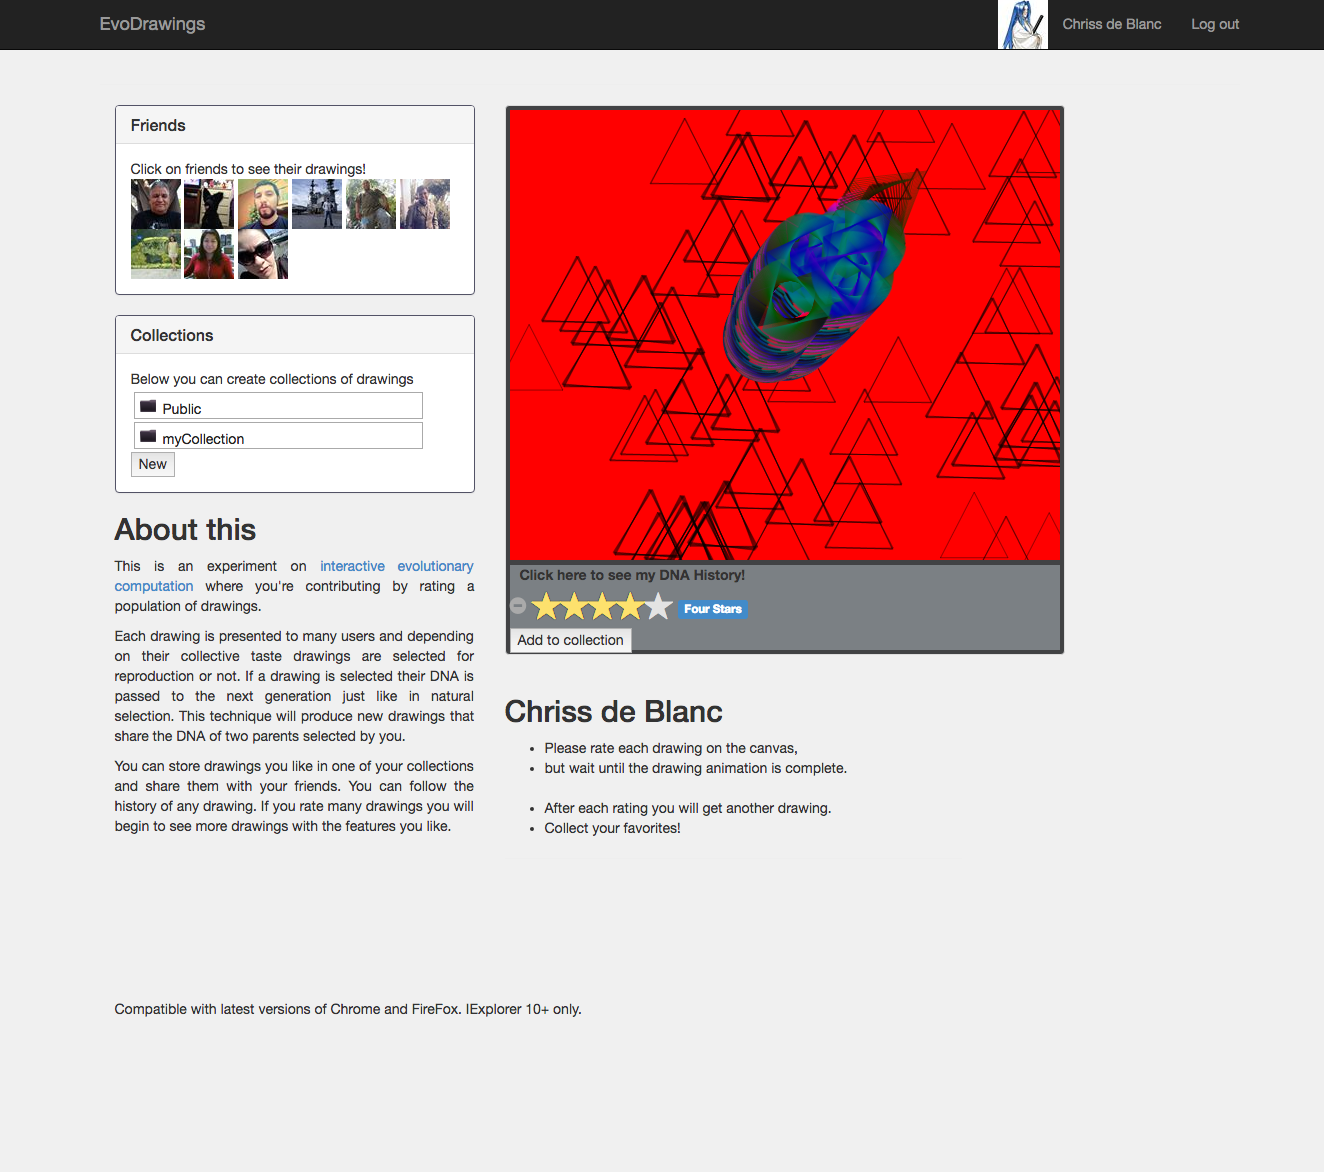
\includegraphics[width=12cm,height=10cm,keepaspectratio]{img/UI_ed01.png}
\caption{User interface ED01.}
\label{fig:UI_01}
\end{figure*}

This detail presents important information about the individual's DNA history,
such as the number of evaluations he has received in the form of likes, the
number of views as well as the ancestry, his genetic crossing operator, the
numerical representation of his chromosome and its identifier within the
population.



\begin{figure*}
\captionsetup{justification=centering,margin=2cm}
\centering
\setlength\fboxsep{0pt}
\setlength\fboxrule{0.7pt}
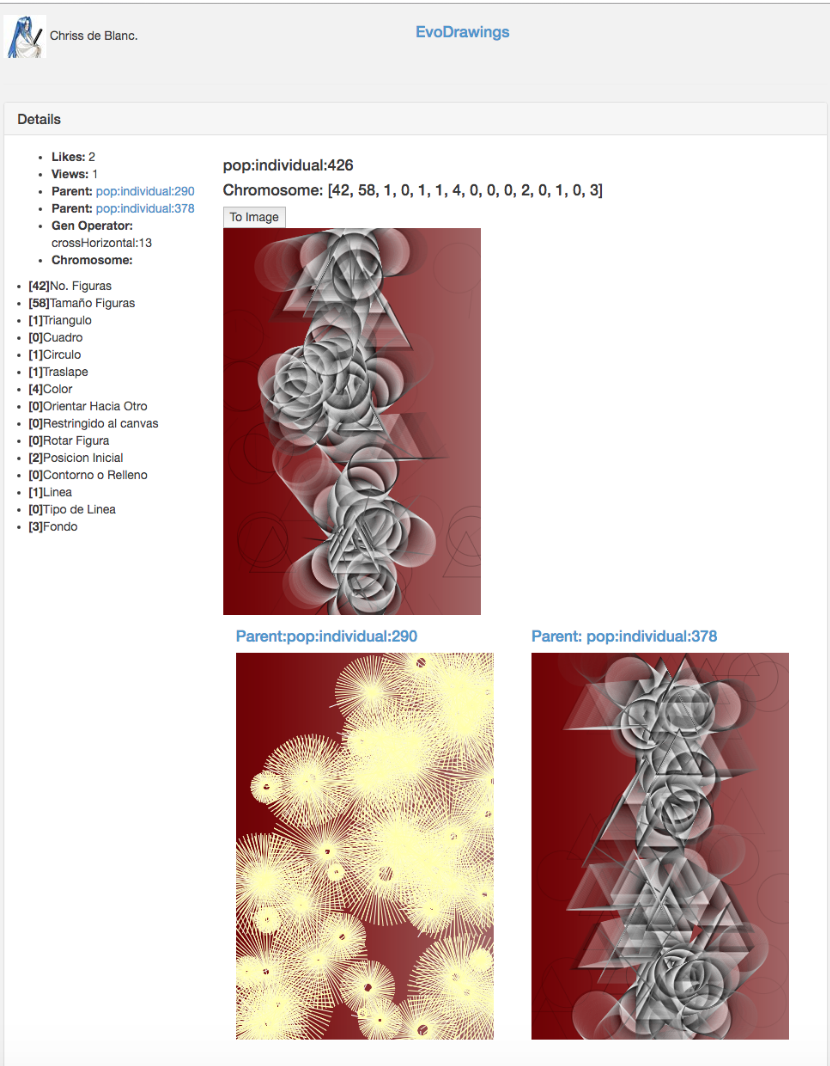
\includegraphics[width=12cm,height=10cm,keepaspectratio]{img/dna.png}
\caption{DNA history.}
\label{fig:dna}
\end{figure*}

For ED02 there is an initial configuration of the interactive evolution
algorithm as follows:

\begin{enumerate}
	\item  \textbf{We have an initial population of 80 individuals.}

	\item  \textbf{An evolution parameter is 8 evaluations.}

	\item  \textbf{A mutation parameter of }
	\item  \textbf{With random selection between competition.}
	\item  \textbf{One horizontal genetic crossing Operator.}
	\item  \textbf{The fitness is given by the equation \ref{eq:fitfunc02}.}
\end{enumerate}

The user interface of this version is the same as the previous version. The
difference between versions lies in how the inference is made internally.

For ED03 there is an initial configuration of the interactive evolution
algorithm as follows:
\begin{enumerate}
	\item  \textbf{We have an initial population of 80 individuals.}

	\item  \textbf{An evolution parameter is 8 evaluations.}

	\item  \textbf{A mutation parameter of }
	\item  \textbf{With random selection between competition.}
	\item  \textbf{One horizontal genetic crossing Operator.}
	\item  \textbf{The fitness is given by the equation \ref{eq:fitfunc02}.}
\end{enumerate}

This version has a new input on the fuzzy functionality named ranking and this
value is given by the cardinality of the graph by each user within the graph-
based user model. Also the fuzzy inference system has a 27 if-then rules which
can visualize in appendix b. The second difference is the usability elements
where the gamification paradigm is apply. Figure \ref{fig:intarface03} shows this
usability elements that are the score level, the experience level and also the
leader board element.

\begin{figure*}
\captionsetup{justification=centering,margin=2cm}
\centering
\setlength\fboxsep{0pt}
\setlength\fboxrule{0.7pt}
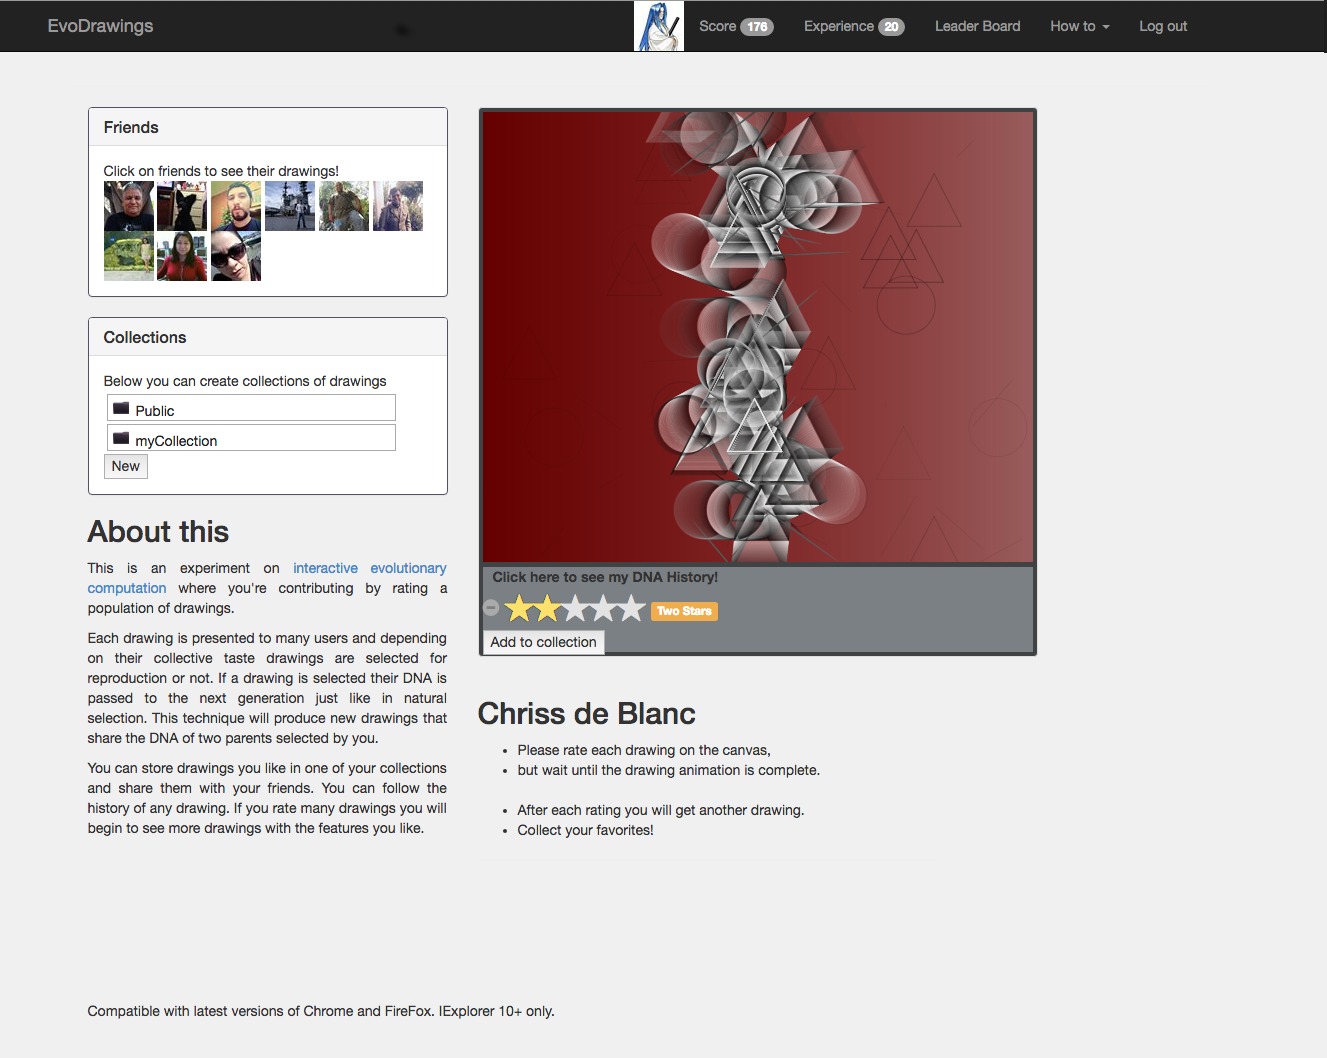
\includegraphics[width=12cm,height=10cm,keepaspectratio]{img/interface.png}
\caption{ED03 Web interface.}
\label{fig:intarface03}
\end{figure*}

This elements in the navigation bar is for users to visualize their scores
inside ED03 application. Likewise the level of experience that is acquiring
through its participations. This version also has an option to see the table of
leaders within the application as shows in Figure \ref{fig:leaderBoard}. This
table shows the 10 best users and the number of entries that have been made so
far.


\begin{figure*}
\captionsetup{justification=centering,margin=2cm}
\centering
\setlength\fboxsep{0pt}
\setlength\fboxrule{0.7pt}
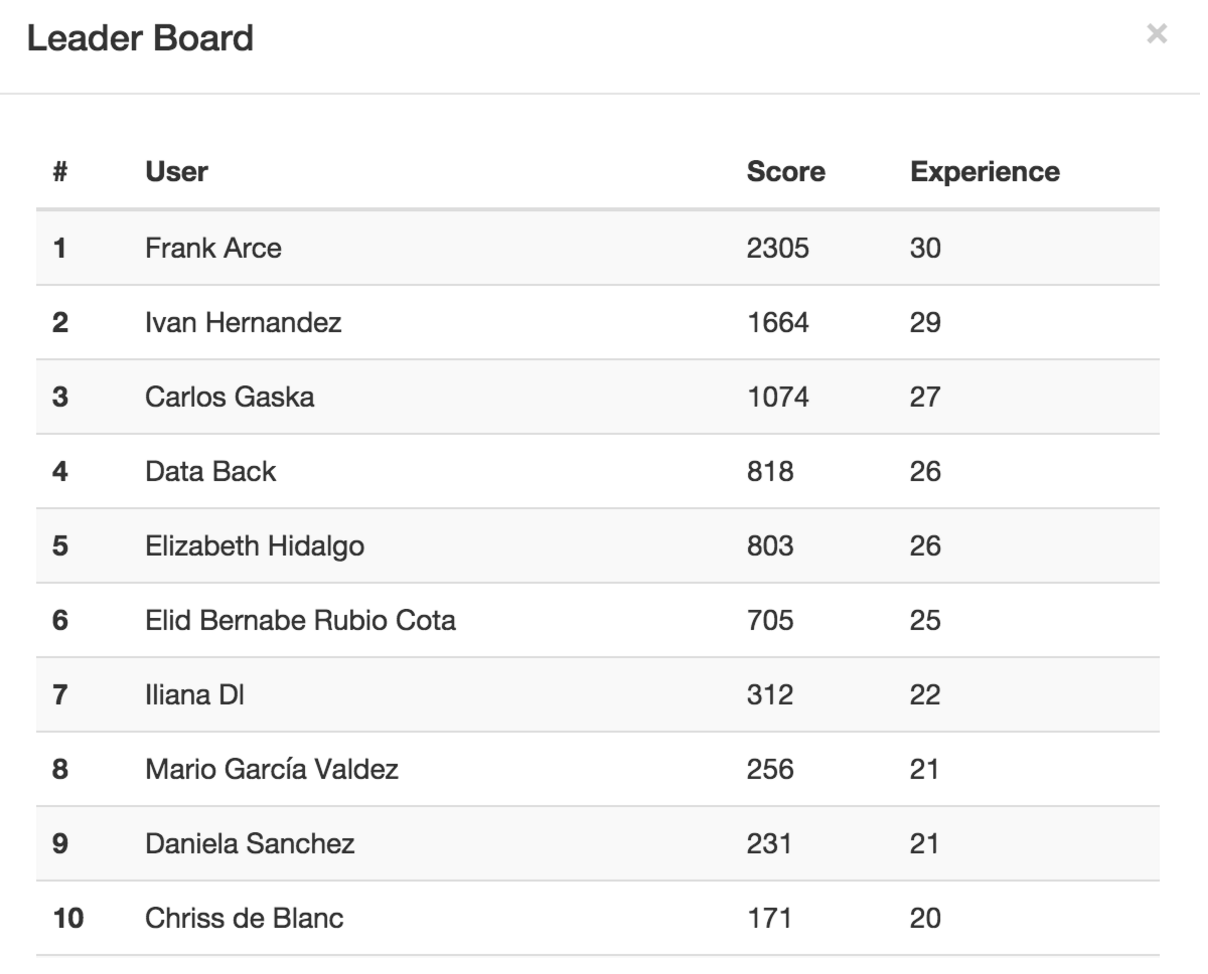
\includegraphics[width=12cm,height=10cm,keepaspectratio]{img/leaderBoard.png}
\caption{Leader board at ED03.}
\label{fig:leaderBoard}
\end{figure*}


\subsection{Promote.}

Each of the experiments was promoted through social networks particularly on
Facebook and Twitter platforms through a short URL as well as an ad to motivate
users to press the link (short URL). This is in order to find participants on a
voluntary basis. This short URL can be seen in table \ref{tab:PromoteUrl}.

\begin{table}
\small
\caption{Short URL for promoting the applicatins.}
\label{tab:PromoteUrl}
\centering
\small
\begin{tabular}{p{5cm} p{4cm}  }
\hline\noalign{\smallskip}
 Long URL & Short URL \\
\noalign{\smallskip}\hline\noalign{\smallskip}
\small{evodrawings01.herokuapp.com } & \small{goo.gl/J8TCe1}  \\ \hline
\small{evodrawings02.herokuapp.com } & \small{goo.gl/jqjNy5}  \\ \hline
\small{evodrawings03.herokuapp.com} & \small{goo.gl/J8TCe1}  \\ \hline
\noalign{\smallskip}\hline
\end{tabular}
\end{table}


\subsection{Heroku dynos and ad-ons server configurations.}
It is necessary to be mentioned that each of the experiments was implemented
under the cloud service (Heroku), in the following Figure \ref{tab:heroku} can
visualize its characteristics by each of the experiments.
\begin{table}
	\small
	\caption{characteristics of  resources and services in cloud Heroku.	}
	\label{tab:heroku}
	\centering
	\small
	\begin{tabular}{p{4cm} p{3cm} p{3cm} p{3cm}  }
		\hline\noalign{\smallskip}
		Service and resources & ED01 & ED02 & ED03 \\
		\noalign{\smallskip}\hline\noalign{\smallskip}
		\small{Heroku Free} & \small{\checkmark} & \small{\checkmark} & \small{\checkmark}\\ \hline
		\small{Deploy from Git} & \small{\checkmark} & \small{\checkmark} & \small{\checkmark}\\ \hline
		\small{Automated patching} & \small{\checkmark} & \small{\checkmark} & \small{\checkmark}\\ \hline
		\small{Self healing apps} & \small{\checkmark} & \small{\checkmark} & \small{\checkmark}\\ \hline
		\small{Undefined logs} & \small{\checkmark} & \small{\checkmark} & \small{\checkmark}\\ \hline
		\small{Number of process types} & \small{2} & \small{2} & \small{2}\\ \hline
		\small{Always on Sleep after 30 mins of inactivity, otherwise always on depending on you remaining mostly free dynes hours} & \small{\checkmark} & \small{\checkmark} & \small{\checkmark}\\ \hline
		\small{Custom domains} & \small{\checkmark} & \small{\checkmark} & \small{\checkmark}\\ \hline
		\small{RAM 512} & \small{\checkmark} & \small{\checkmark} & \small{\checkmark}\\ \hline
		\small{Dedicated} & \small{x} & \small{x} & \small{x}\\ \hline
		\small{Heroku Postgres ::DB Hobby Dev} & \small{\checkmark} & \small{\checkmark} & \small{\checkmark}\\ \hline
		\small{GrapheneDB Chalk} & \small{\checkmark} & \small{x} & \small{\checkmark}\\ \hline
		\small{Redis To Go Nano} & \small{\checkmark} & \small{x} & \small{\checkmark}\\ \hline
		\small{GrapheneDB Sandstone} & \small{x} & \small{x} & \small{\checkmark}\\ \hline
		\small{Redis To Go Mini} & \small{x} & \small{x} & \small{\checkmark}\\ \hline


		\noalign{\smallskip}\hline
	\end{tabular}
\end{table}


The initial purpose of the experiments is to design specific applications and
interfaces to enable users to participate voluntarily within the different
applications. Each experiment allowed the task of collecting data that will
later be analyzed to determine which of these versions had the largest number of
user participations. To verify the initial hypothesis, 3  versions were implemented with
slight differences in the configuration characteristics of each application,
which allowed to decide through the results obtained which of them verify the
hypothesis of this investigation. The results obtained
are presented in the next chapter.
